\documentclass[11pt]{article}
\author{Lawrence Liu}
\usepackage{subcaption}
\usepackage{graphicx}
\usepackage{amsmath,amssymb,stmaryrd}
\usepackage{physics}
\usepackage{pdfpages}
\newcommand{\Laplace}{\mathscr{L}}
\setlength{\parskip}{\baselineskip}%
\setlength{\parindent}{0pt}%
\usepackage{xcolor}
\usepackage{listings}
\definecolor{backcolour}{rgb}{0.95,0.95,0.92}
\usepackage{amssymb}
\lstdefinestyle{mystyle}{
    backgroundcolor=\color{backcolour}}
\lstset{style=mystyle}
\title{Physics 115C HW 3}
\begin{document}
\maketitle
\section*{Problem 1}
\subsection*{(a)}
Since the ground state should have no nodes, we would expect it to be 
symmetric. And since the first excited state should have 
be orthogonal to the ground state, we would expect it to be antisymmetric.
Therefore a rough sketch of the wavefunctions would be:
% \begin{figure}[h]
%     \centering
    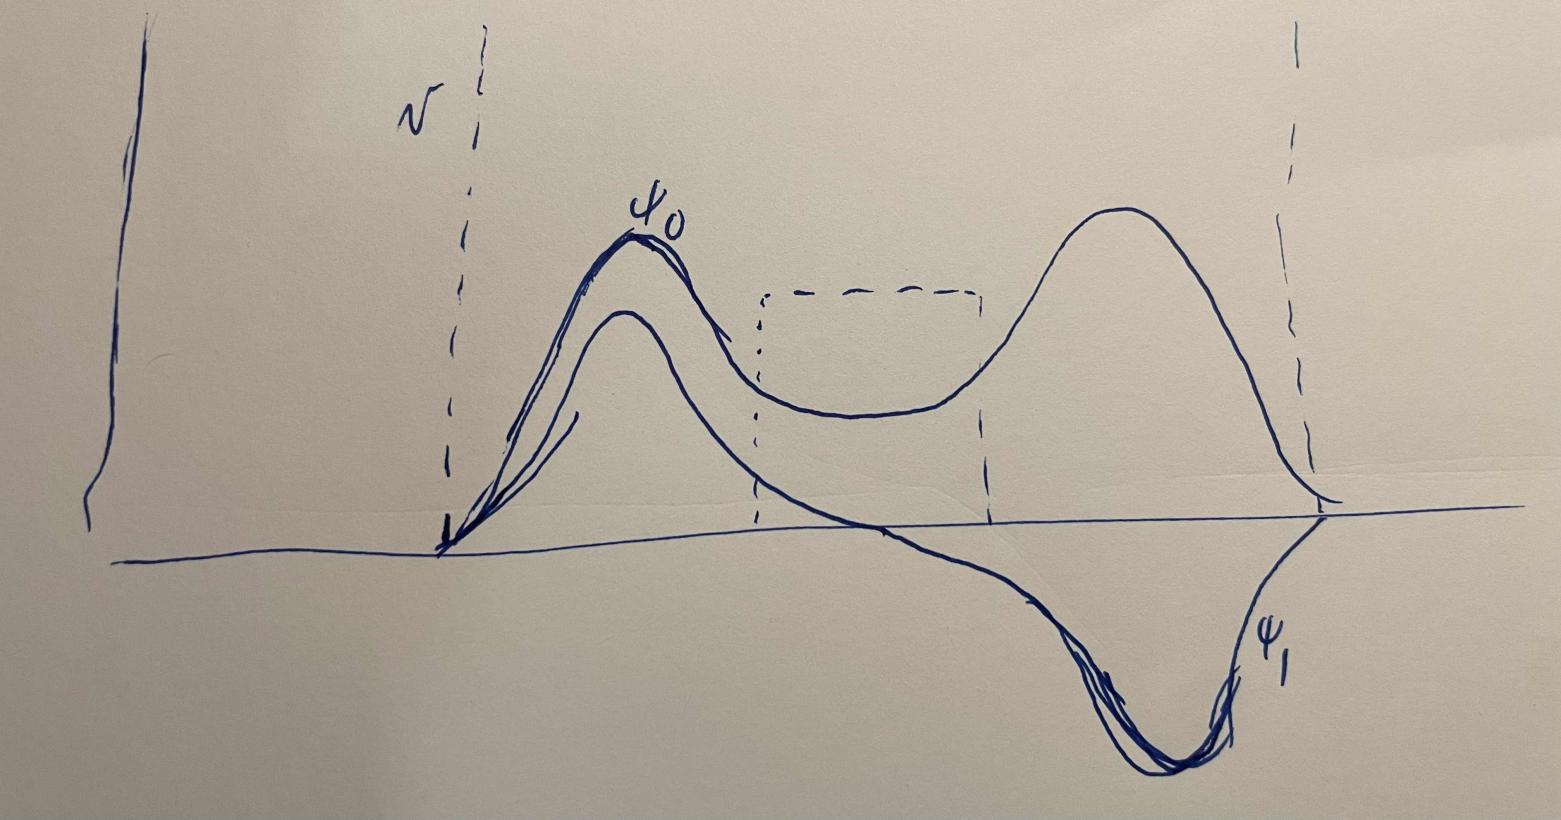
\includegraphics[width=0.5\textwidth]{prob1a.png}
%     \caption{Sketch of the ground state and first excited state wavefunctions}
% \end{figure}
\subsection*{(b)}
We have that if the central barrier height is $0$, then the problem becomes the 
infinite square well problem. Therefore the ground state and first excited state
are:
\includegraphics*[width=0.5\textwidth]{prob1b1.png}
And if the central barrier height is $\infty$, then the particle cannot exist in the 
center. Therefore the ground state and first excited state are:
\includegraphics*[width=0.5\textwidth]{prob1b2.png}
Thus we can see that the splitting will be large when the central barrier is close to $0$, and 
large when the central barrier is close to $\infty$.
\subsection*{(c)}
\includegraphics*[width=0.5\textwidth]{prob1c.png}
\subsection*{(d)}
The $\psi_{\pm}(x)$ wavefunctions are not parity symmetric. However the Hamilonian is 
parity symmetric.
\subsection*{(e)}
The expectation value of $\bra{\psi_{+}}x\ket{\psi_{+}}$ and 
$\bra{\psi_{-}}x\ket{\psi_{-}}$ are bot not $0$ since $\psi_{\pm}(x)$ is 
not parity symmetric. However the expectation value of $
\bra{\psi_{0}}x\ket{\psi_{0}}$ and $\bra{\psi_{1}}x\ket{\psi_{1}}$ are $0$ since 
$\psi_{0}(x)$ and $\psi_{1}(x)$ are parity symmetric.
\subsection*{(f)}
No in the case of finite barrier height we will have that $\ket{\psi_0}$ 
and $\ket{\psi_1}$ will no longer be degenerate. Therefore they will evolve at 
different rates, and thus $\ket{\pm}$ will no longer be stationary states.
\subsection*{(g)}
$$\ket{+(t)} = \frac{1}{\sqrt{2}}\left(
    e^{-iE_0t/\hbar}\ket{0} + e^{-iE_1t/\hbar}\ket{1}
\right)$$
\subsection*{(h)}
The probability that the particle is in state $\ket{-}$ is given by 
\begin{align*}
    |\bra{-}\ket{+(t)}|^2 &= \frac{1}{4}\left|
        e^{-iE_0t/\hbar} + e^{-iE_1t/\hbar}\right|^2\\
        &= \frac{1}{4}\left(
            (\cos(\frac{E_0t}{\hbar}) + \cos(\frac{E_1t}{\hbar}))^2 + 
            (\sin(\frac{E_0t}{\hbar}) + \sin(\frac{E_1t}{\hbar}))^2
        \right)\\
        &= \frac{1}{4}\left(
            2 + 2\cos(\frac{(E_0 - E_1)t}{\hbar})\right)
\end{align*}
Therefore we can see that the first time particle will turn 
into state $\ket{-}$ is when $t = \frac{\pi\hbar}{E_1 - E_0}$.
\subsection*{(i)}
As we raise the barrier height, the splitting between the ground state and 
the first excited state will decrease therefore 
the time it takes for the particle to turn into state $\ket{-}$ will increase. And when 
the barrier height becomes infinite, the particle will never turn into state $\ket{-}$. 
\subsection*{(j)}
$$\frac{2\pi\hbar}{E_1-E_0} = \frac{1}{24\cdot10^9}$$
$$E_1-E_0 = 1.590\cdot 10^{-23}J$$
The wavelength of the light emited is given by 
$$\lambda = \frac{hc}{E_1-E_0} = 0.012m$$
Therefore we can see that the wavelength of the light emited is in the
microwave range. 
\subsection*{(k)}
The time it would take to tunnel is 
$$\frac{1}{2\cdot 160\mu \text{Hz}} = 3125s$$
This tunneling time is much longer than Ammonia, therefore we can conclude 
that the barrier height for $AsH_3$ is much higher than that of Ammonia.
\subsection*{(l)}
It would depend how long the measurement is taken. Both atoms have an "instantenous" dipole,
ie if we measure instantenously, we will find that the dipole is non-zero, since the 
As or N atom will be on one side of hydrogen plane. But when
the As or N atom oscillates to the other side of the hydrogen plane, the dipole will flip.
So the net dipole if we measure for a long time (on the order of days) will be $0$.
\section*{Problem 2}
\subsection*{(a)}


\end{document}
 
